\documentclass[pdf,slideColor,fyma]{beamer}
 	\usepackage[utf8]{inputenc}
	\usepackage[IL2]{fontenc}
	\usepackage[czech]{babel}
	\usepackage{graphicx}

\usecolortheme{crane}
\title{Binárna sústava}
	\author{Vladimír Marcin \\ 
		{\footnotesize xmarci10@stud.fit.vutbr.cz}}	
	\institute{Fakulta informačních technologií \\ 
						 Vysoké učení technické v~Brně}
	\date{\today}

\begin{document}
\begin{frame}
	\titlepage
\end{frame}

\begin{frame}
\frametitle{Motivácia}
Ľudí možno rozdeliť do 10 skupín\,--\,na tých, ktorí rozumejú
binárnej sústave a~ktorí jej nerozumejú.
\medskip
\begin{figure}[h]
	
\includegraphics[height=1.5cm]{smile.png}
	\centering
\end{figure}
\end{frame}

\begin{frame}
\frametitle{Dvojková číselná sústava}
	\begin{itemize}
		\item dvojková (binárna) číselná sústava má význam od obdobia vzniku elektronických počítačov,
		\item elektronické konštrukčné prvky počítačov majú dva stabilné stavy,
		\item tieto fyzikálne prvky svojou činnosťou priamo modelujú znaky dvojkovej číselnej sústavy,
		\item všetky informácie aj v~súčasnom počítači sú uložené pomocou dvoch znakov: \textbf{0} a~\textbf{1}
	\end{itemize}
\medskip
\large{Základnú jednotku informácie nazývame \textbf{1 bit} (binary digit).}
\end{frame}

\begin{frame}
\frametitle{Dvojková číselná sústava}
\begin{itemize}
	\item Základ:\hspace{5.1em} $2$
	\item Používané číslice:\hspace{1em} $0, 1$
	\item Mocniny základu:\hspace{1em} $2^0, 2^1, 2^2, 2^3,$\dots
\end{itemize}
\medskip
\textbf{Binárny zápis čísla:}\\
\medskip
$1101101_2=1*2^0+0*2^1+1*2^2+1*2^3+0*2^4+1*2^5+1*2^6$
\end{frame}

\begin{frame}
\frametitle{Binárny zápis čísla}
\begin{itemize}
	\item na zápis v~dvojkovej sústave používame iba číslice 0 a~1,
	\item každá pozícia v~zápise daného čísla predstavuje inú mocninu základu tejto sústavy\,--\,teda inú mocninu čísla 2.
\end{itemize}
\begin{figure}[h]
	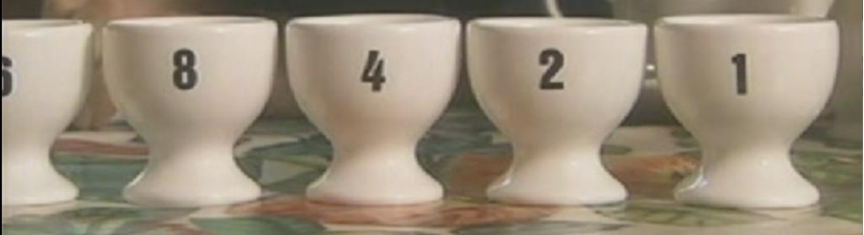
\includegraphics[height=2.5cm]{no_eggs.png}
	\centering
\end{figure}
\end{frame}

\begin{frame}
\frametitle{Binárny zápis čísla}
\begin{itemize}
	\item Pr.: Číslo 9 má v binárnej sústave podobu 1001, čo odpovedá obsadeným pozíciám v~obrázku. Číslo 9 totiž vieme zapísať ako $8+1=2^3+2^0$.
\end{itemize}
\begin{figure}[h]
	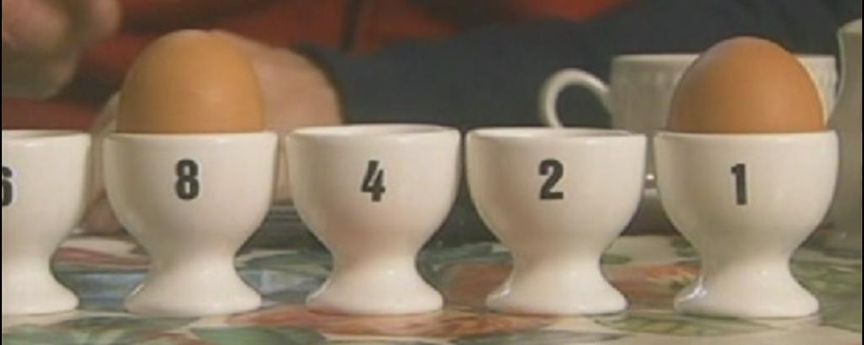
\includegraphics[height=3cm]{eggs.png}
	\centering
\end{figure}
\end{frame}

\begin{frame}
\frametitle{Aritmetické operácie v~dvojkovej sústave}
\begin{itemize}
	\item pravidlá pre vykonávanie aritmetických operácií si treba osvojiť len pre dve číslice, ktoré sa môžu vyskytnúť v~jednom ráde
	\item pravidlá pre aritemtické operácie v~dvojkovej sústave sú nasledujúce:
\end{itemize}
\medskip
\begin{center}
\begin{tabbing}
Odčítanie:\qquad \= Odčítanie:\qquad \= Odčítanie:\qquad \= Odčítanie\qquad \kill
\>\textbf{Sčítanie:} \>\textbf{Odčítanie:} \>\textbf{Násobenie:}\\
\>$0+0=0$ \> $0-0=0$ \> $0*0=0$\\
\>$0+1=1$ \> $1-0=1$ \> $0*1=0$\\
\>$1+0=1$ \> $1-1=0$ \> $1*0=0$\\
\>$1+1=10$\> $10-1=1$\> $1*1=1$
\end{tabbing}
\end{center}
\end{frame}

\begin{frame}
\frametitle{Zdroje}
	\begin{itemize}
		\item Dvojková číselná sústava,\\
		\url{https://sk.wikipedia.org/wiki/Dvojková\_číselná\_sústava}
		\item Pozičné číselné sústavy,\\
		\url{http://www.bilgym.sk/data/2011-2012/Maths/pozicne\_ciselne\_sustavy.pdf}
	\end{itemize}
\end{frame}

\end{document}
